\documentclass{article}
\usepackage{graphicx} % Required for inserting images

\title{Dark Star -- Communicating with Distant Solar Systems from Earth with Cubesat Starshade Swarms that Occult Passing Starlight.}
\author{Leonardo Armel, Robert G Kennedy III, and Jeff Shrager*}\thanks{Authors listed alphabetically. LA is at Gunn High School, Palo Alto, CA. RGK is at XXX, and JS is at Blue Dot Change and Consulting Professor in the Symbolic Systems Program at Stanford University.
}
\date{January 2024}
\begin{document}
\maketitle

\section{Concept}

Generating a spatially-coherent photon beam that can reliably transmit information through interstellar space requires an impractical amount of power. However, there is already a set of extremely powerful, spatially coherent, point-sources that are known to travel millions of light years through interstellar space that we can piggy-back on to send interstellar messages. Specifically, an observer in, say, the Alpha Centauri system, looking at our system through even a moderately powerful telescope, will see continuous and spatially coherent light arriving from hundreds or even thousands of distinct stars that are behind our system relative to the observer  in Alpha Centauri, but whose light is passing through our system on its way to that observer. We propose that a carefully coordinated swarm of very small spacecraft, deployed throughout our solar system, and both powered and navigated by active attitude control of their solar collectors, could dynamically occult selected beams passing from Sol to Centauri in order to create a binary signal that would be clearly visible to the remote observer as "oddly twinkling” stars.

The Centauri system makes a convenient analog to ours as the separation between the two brighter stars, $\alpha$ Centauri A and B, varies from roughly 10 to 40 AU, which is roughly the distance between our sun and Pluto. Separation between the A/B pair and the third member of the system, Proxima Centauri, is roughly 10,000 AU, comparable to the distance from our Sun to well into its Oort Cloud.  Therefore, picturing the Centauri system gives us a good sense of the field of view that a remote observer will see when they look at us from there. Figure 1 is a photograph from wikimedia of the Centauri system taken with a common zoom lens (85mm) and with uncomplicated photographic protocol ("Canon 85mm f/1.8 lens with 11 frames stacked, each frame exposed 30 seconds" [url]]). 
\begin{figure}
    \centering
      \makebox[\textwidth]{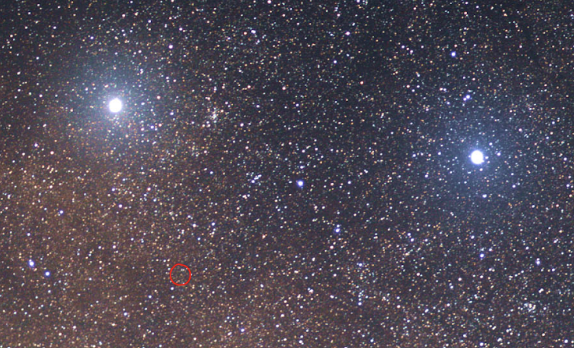
\includegraphics[width=\textwidth]{Fig1.png}}
        \caption{The $\alpha$ Centauri system. footnote: Source: $https://en.wikipedia.org/wiki/Alpha_Centauri/media/File:Alpha,_Beta_and_Proxima_Centauri_(1).jpg$ Cropped for emphasis.}
    \label{fig:1_centauri_system}
\end{figure}

There are easily several hundred clearly distinct point sources whose light passed though the Alpha Centauri system around 4 ly ago, and reached Earth to be captured in this photograph. An observer on a planet in the Alpha Centauri system photographing our solar system would see a similar palette of point sources.\footnote{Centaurus is in the densest part of the milky way, from our point of view, so looking at the Alpha Centauri system from earth we will see many more background stars than someone in the Alpha Centauri system would see looking at us, out here on the edge of the galaxy. Nonetheless, there are still hundreds of such stars from the opposite point of view, and the present proposal only requires, in the extreme, one star visible through the source system.}

The present proposal is to deploy a swarm of small robotic spacecraft, which we shall call "Dark Stars", controlled from Earth and both powered and propelled by their solar cells, which double as light sails.[cite Dyson Dots here:\footnote{Kennedy, Robert G., Eric Hughes, Kenneth I, Roy, and David E. Fields. 2013. Dyson Dots and Geoengineering: the Killer App Ad Astra. Tennessee Valley Interstellar Workshop 2013 Special Issue of Journal of the British Interplanetary Society, volume 66, no. 10-11, pages 340-358. Oct/Nov 2013.  Bibcode: https://ui.adsabs.harvard.edu/abs/2013JBIS...66..340K/abstract} ]  Turning the cells in various directions enables the Dark Star to maneuver slowly through the solar system, while Earth-based laser PNT (position-navigation-timing)[cite laser nano-bot positioning paper] could be used in initial deployment aid in positioning, if faster movement is required.\footnote{Because the Dark Stars are unpowered, positioning can only be done away from the sun or earth, but the starlight blocking method does not depend upon the swarm being particularly close to earth, except as regards unacceptable communications delays, but this can be algorithmically compensated.}  

\section{Universal Dynamic Targeting}

If they are deployed approximately evenly through our solar system, the Dark Star swarm can be used to target messages in any desired direction (Fig. 2).

\begin{figure}
    \centering
      \makebox[\textwidth]{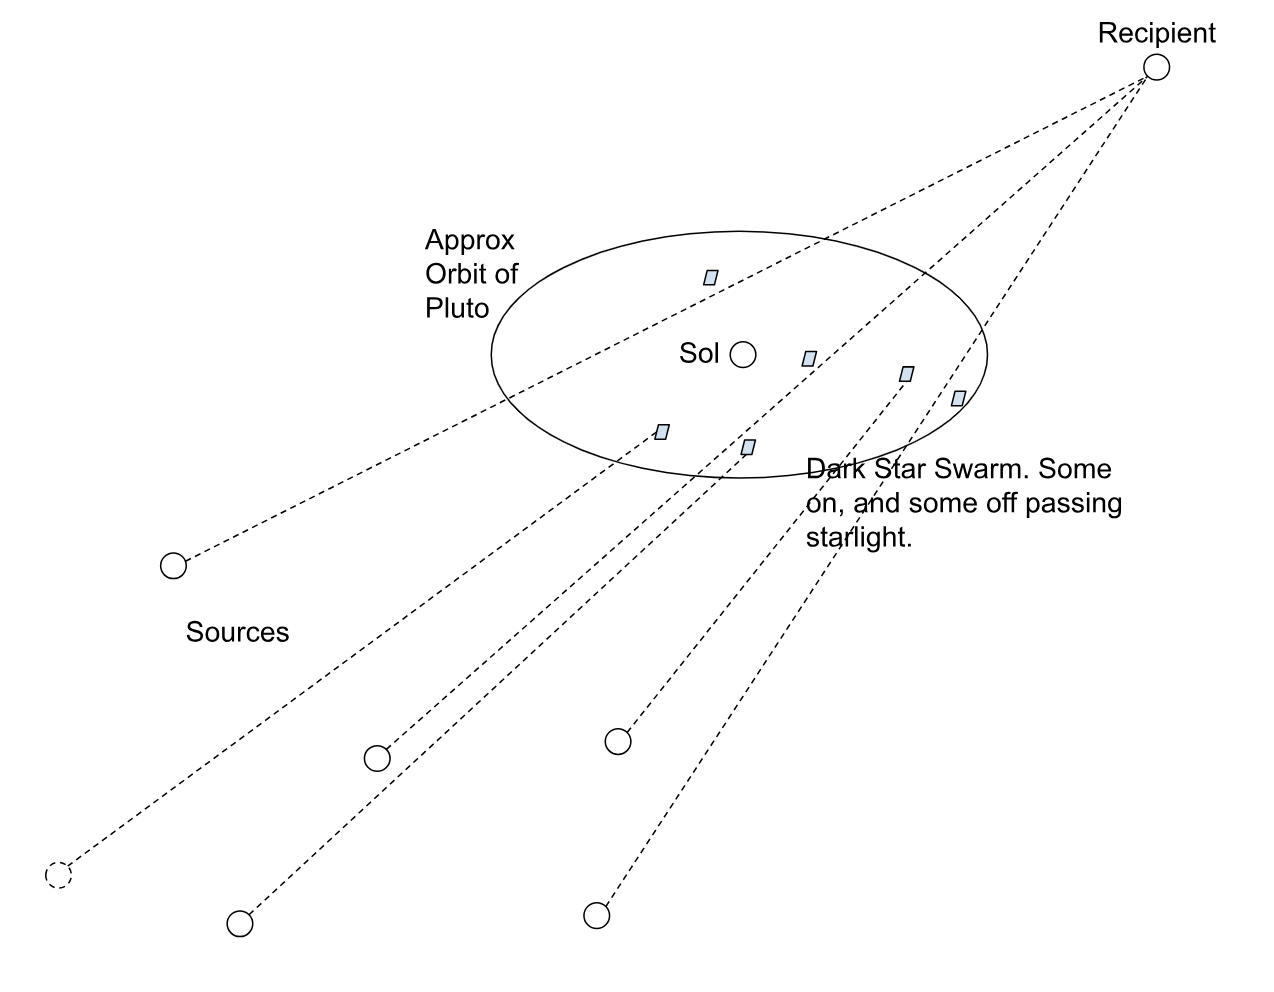
\includegraphics[width=\textwidth]{Fig2.png}}
    \caption{}
    \label{fig:1_centauri_system}
\end{figure}

\section{Aspects of Positioning - Jibing Through the Starlight}

In our conception, each Dark Star has two cameras located on opposite sides of the craft from one another. These are used for positioning. As the Dark Stars are always moving away from the sun, but the sun itself is not a source beam (as it is far too close, and thus too large, to be used as a source beam), the crafts must block their assigned source beam by metaphorically jibing back and forth across it (Fig. 3). 

\begin{figure}
    \centering
      \makebox[\textwidth]{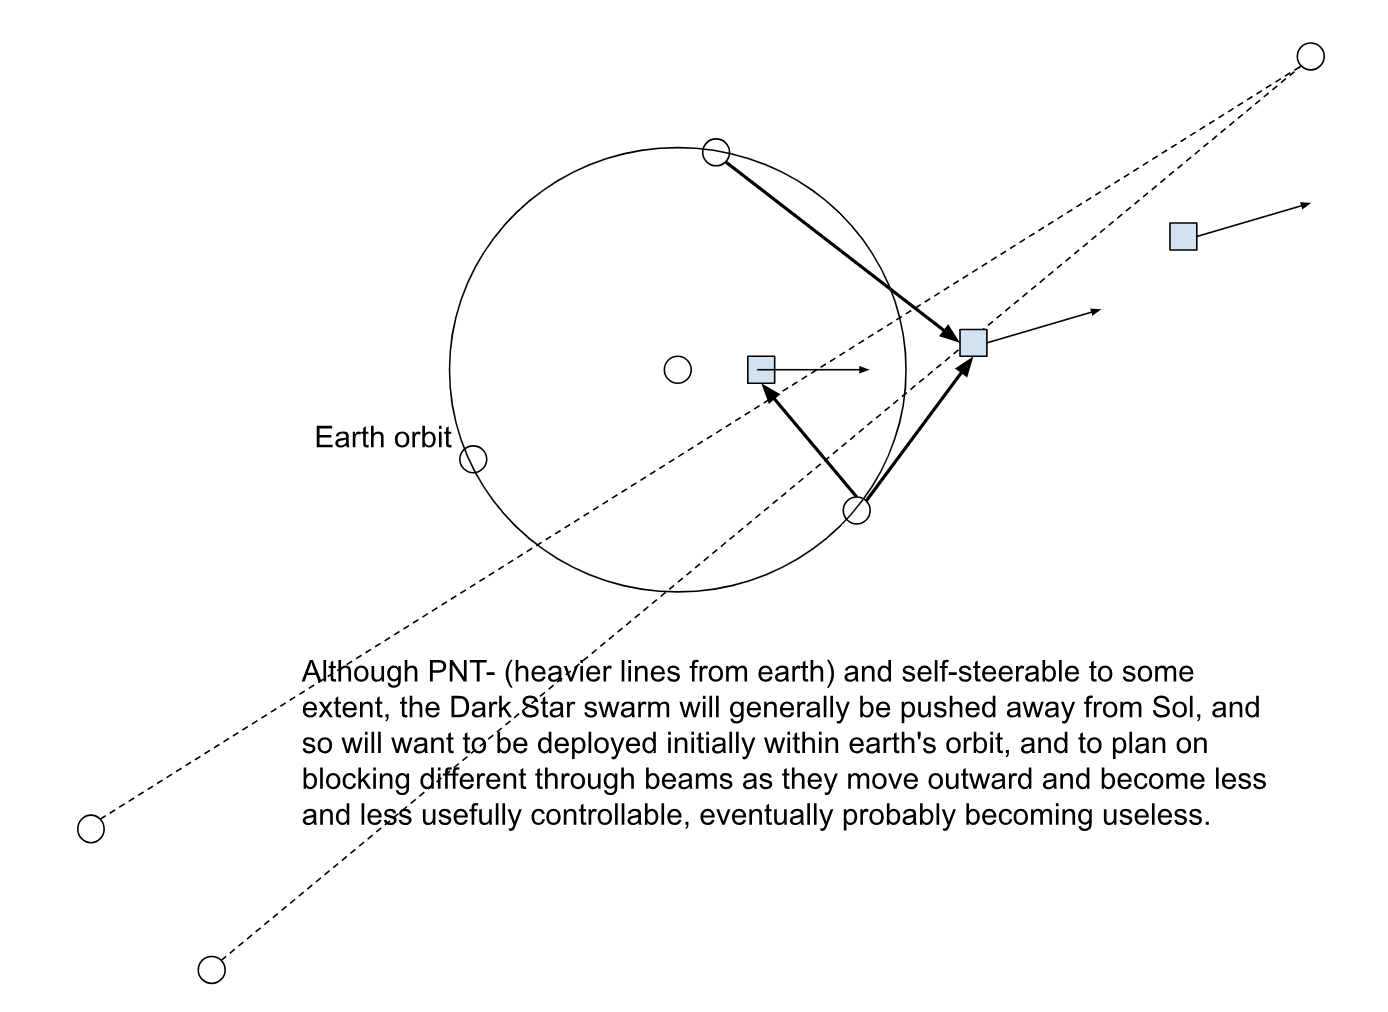
\includegraphics[width=\textwidth]{Fig3.png}}
    \caption{}
    \label{fig:3_jibing}
\end{figure}

\section{Multiple Targeting}

\begin{figure}
    \centering
      \makebox[\textwidth]{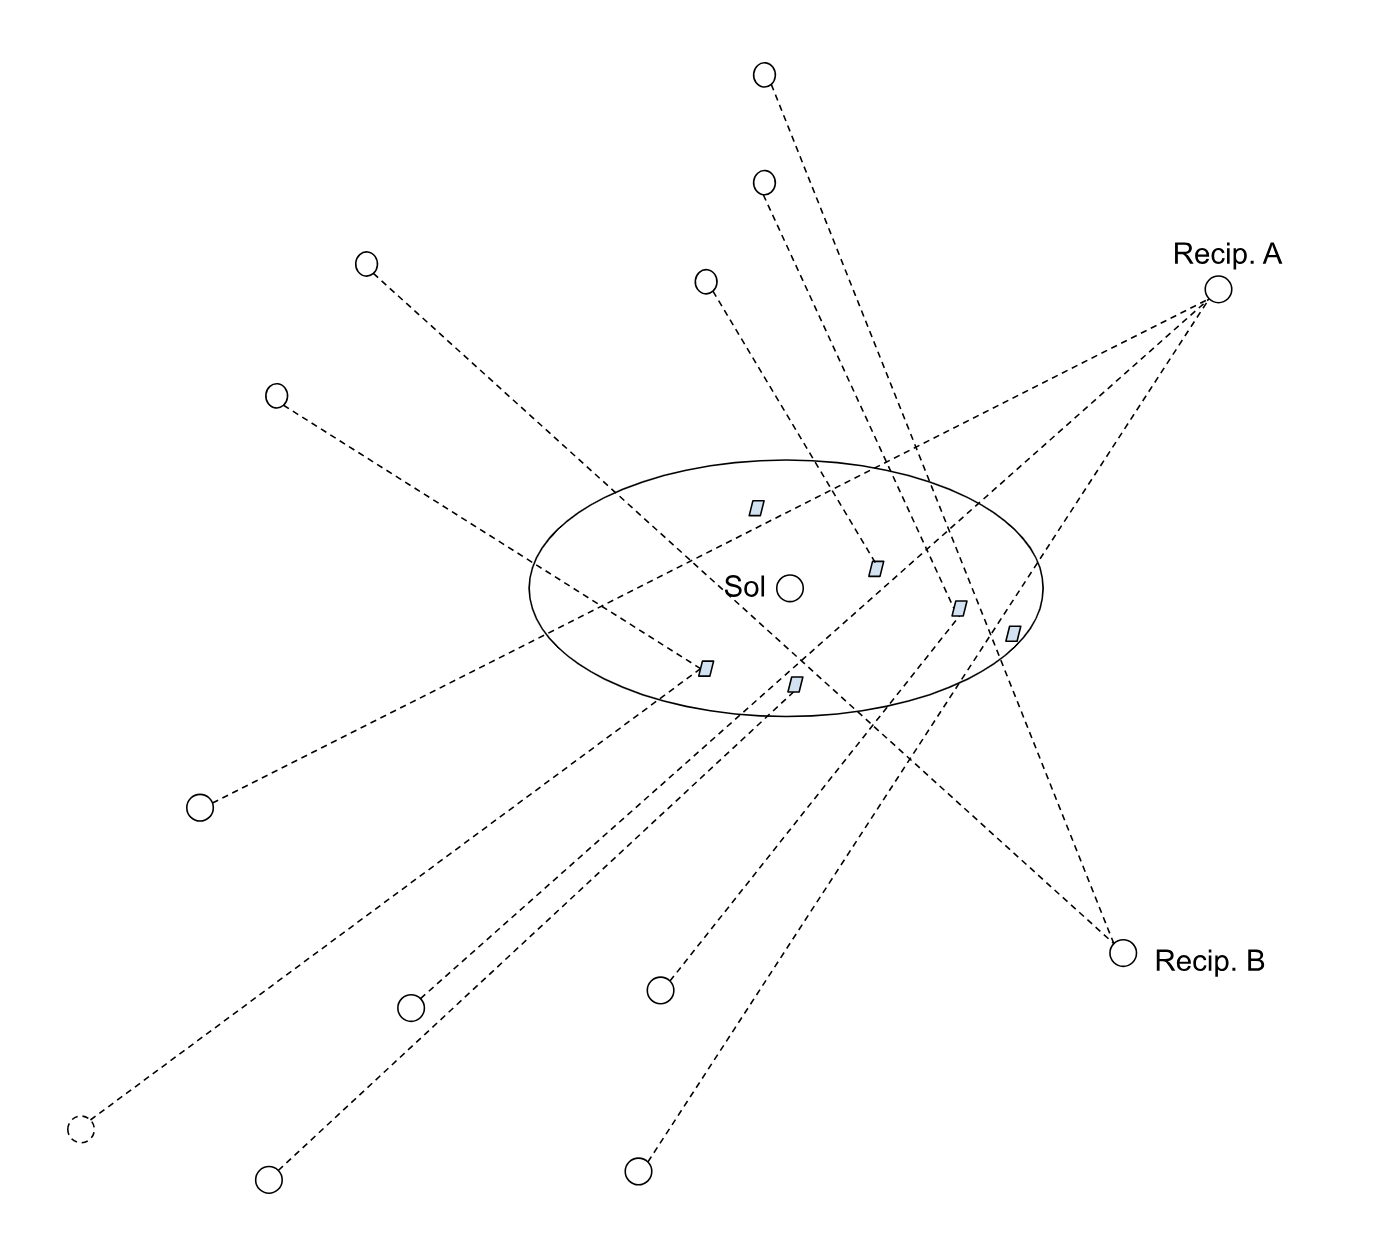
\includegraphics[width=\textwidth]{Fig4.png}}
    \caption{}
    \label{fig:4_multitargets}
\end{figure}


\end{document}
